\section*{Swapping Policies (minimize cache miss/page fetch)}
\begin{itemize}
\item Average Memory Access Time (AMAT)=$T_{M}+(P_{\text{Miss}} + T_{D})$
\item $T_{M}$ the cost of accessing memory; $T_{D}$ the cost of accessing disk
\item $P_{\text{Miss}}$ the probability of not finding  data in cache (a miss) [0.0,1.0]
\item $P_{\text{Miss}} = 0.1$, $T_{D}=10$ms, $T_{M}$=100ns $\to$ AMAT = 1.0001ms
\item $P_{\text{Miss}} = 0.001$ ($P_{\text{Hit}} = 0.999$) $\to$ AMAT = 10.1$\mu$s (100 times faster)
\item In general, $P_{\text{Miss}} + P_{\text{Hit}} = 1.0$
\end{itemize}

\section*{Types of cache misses (3 categories)}
\begin{enumerate}
\item compulsory miss (aka cold-start miss): cache is empty (first reference)
\item capacity miss: no enough space $\to$ evict old to make room for new
\item conflict miss: arises due to (hardware) limits on where the item can be placed in cache.  Conflict miss doesn’t occur in the OS page cache, as the cache is
fully associative (a page can be placed anywhere)
\end{enumerate}

\section*{The optimal policy (by Belady), FIFO, Random, LRU, LFU}
\begin{itemize}
\item replace the page that will be accessed \textbf{furthest in the future}
\item Hard to implement (because hard to predict the future)
\item Useful as an ideal policy to compare with (can't do better than optimal)
\end{itemize}
\begin{itemize}
\item FIFO/Random: might evict important pages (to be ref-ed again soon)
\item \textbf{frequency} a page accessed frequently is perhaps important
\item \textbf{recency} a page accessed recently will perhaps be accessed again
\end{itemize}
\section*{Workload examples (100 unique pages)}
\begin{minipage}{0.33\linewidth}
  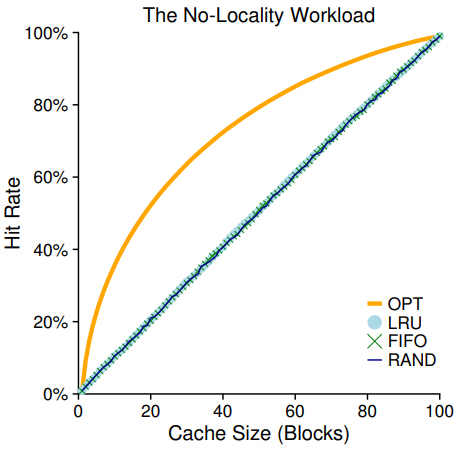
\includegraphics[width=\linewidth,height=3.5cm]{imgs/non_locality_workload}
\end{minipage}
\begin{minipage}{0.34\linewidth}
  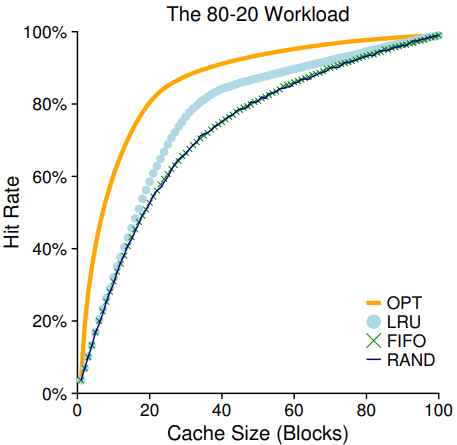
\includegraphics[width=\linewidth,height=3.5cm]{imgs/eight_20_workload}
\end{minipage}
\begin{minipage}{0.33\linewidth}
  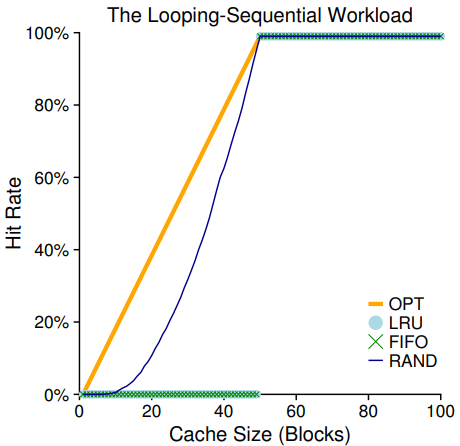
\includegraphics[width=\linewidth,height=3.5cm]{imgs/looping_workload}
\end{minipage}
\begin{minipage}{0.5\linewidth}
  \flushleft
  \begin{enumerate}
  \item no locality $\to$ any policy works
  \item when cache size $>$ workload, swap policy in use doesn't matter
  \item optimal performs better than other realistic policies
  \item for 80-20, LRU does better than random/FIFO
  \end{enumerate}
\end{minipage}
\begin{minipage}{0.5\linewidth}
  \flushleft
  \begin{enumerate}
  \item loops common in applications (eg databases)
  \item worst case scenario for FIFO and LRU
  \item A looping workload with N pages and cache size $<$ N pages always result in
0\% hit rate
  \end{enumerate}
\end{minipage}

\section*{Issues of implementing LRU}
\begin{itemize}
\item implementing history-based policies requires accounting of every memory ref $\to$ performance $\downarrow$ if not careful
\item possible hardware support: update time field in memory for each page
\item OS then scans time fields to find LRU page: expensive if page num $\uparrow$
\end{itemize}
\section*{Approximating LRU: clock algorithm}
\begin{itemize}
\item use a \textbf{use bit} (aka \textbf{reference bit} to page)
\item when page is accessed, set bit to 1 (done by hardware)
\item arrange all pages in a circular list and when replacement occurs
\item if use bit is 1, set it to 0 and move on; if use bit is 0, evict the page
\end{itemize}
\section*{Dirty Pages (regarding clock algorithm: whether a page is modified)}
\begin{itemize}
\item If page has been modified, do not evict (write to disk is expensive)
\item If page is clean, eviction is free (no need to write to disk)
\item hardware support should include a \textbf{dirty bit}
\end{itemize}
\section*{Belady's anomaly}
\begin{itemize}
\item In general, cache size $\uparrow \to$ cache hit rate $\uparrow$ but not true for FIFO
\item stack property: For algorithms (eg LRU) with this property, cache of size N + 1 naturally includes contents of a cache of size N
\item FIFO/Random (among others) do not obey the stack property; susceptible to anomalous behavior
\end{itemize}
